\documentclass[a4paper]{article}
\usepackage[utf8]{inputenc}
\usepackage[T1]{fontenc}
\usepackage{graphicx}
\usepackage{hyperref}
\usepackage[a4paper, %showframe,
            twoside, includehead,
            footskip=7mm, headsep=6mm, headheight=4.8mm,
            marginparsep=2mm, marginparwidth=22mm,
            top=25mm, bottom=25mm, inner=30mm, outer=25mm]{geometry}
\usepackage{sansmathfonts}
\usepackage[section]{placeins}
\usepackage{fancyhdr}
\usepackage[spanish, es-tabla, es-nodecimaldot]{babel}

\fancypagestyle{plain}{
  \fancyhf{}%
  \fancyfoot[R]{\thepage}
}
\pagestyle{plain}
\renewcommand{\headrulewidth}{0pt}
\renewcommand{\footrulewidth}{0.5pt}

\hypersetup{
    colorlinks=true,
    linkcolor=blue,
    filecolor=magenta,      
    urlcolor=blue,
}
\urlstyle{same}

\title{Informe de Avance - Proyecto Karting 2019}
\author{Dr. Ing. Pablo Cossutta}
\date{Junio 2019}

\begin{document}
\maketitle
%
\section{Introducción}
El proyecto denominado Karting Eléctrico es multidisciplinario ya que convergen varias disciplinas diferentes como electrónica, informática y mecánica. Dentro del ámbito electrónico, involucra a varias áreas de la misma como por ej. el desarrollo de convertidores de potencia, sistemas de control, modelado e identificación y comunicaciones entre otras.

El objetivo principal de este proyecto es proveer al ITBA de una plataforma de movilidad eléctrica experimental de tracción integral, donde toda la electrónica esté desarrollada en el propio instituto con el fin de impulsar los trabajos de investigación relacionados con movilidad eléctrica. Dentro de las posibles áreas de investigación se encuentra el diseño y control de convertidores para motores eléctricos del tipo BLDC, control de tracción y estabilidad de vehículos eléctricos y desarrollo de sistemas de carga rápida de baterías.

Con este objetivo en mente y teniendo en cuenta las restricciones de espacio se procedió a desarrollar un prototipo de karting eléctrico de tracción integral basado en un chasis tradicional. La plataforma experimental realizada se observa en la Fig. \ref{fig:kart1}.
\begin{figure}[h]
    \centering
    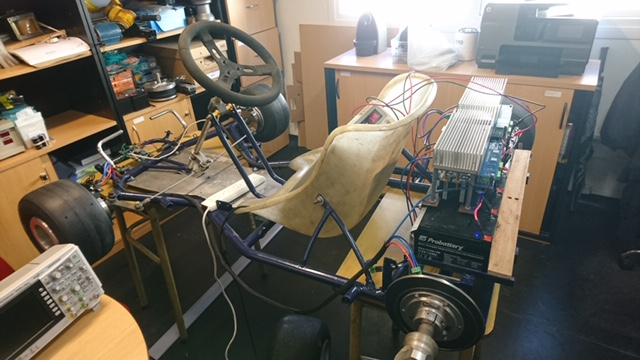
\includegraphics[width=0.7\textwidth]{figs/kart1.jpg}
    \caption{Prototipo de Karting eléctrico}
    \label{fig:kart1}
\end{figure}

Los trabajos realizados incluyen desde el diseño y construcción de las llantas que incluyen los motores de las ruedas delanteras hasta el diseño y control de los convertidores electrónicos de potencia, pasando por el dimensionamiento de los cableados y la instalación de los mismos. En la Fig. \ref{fig:kart2} puede observarse el estado actual de construcción del prototipo.
%
\begin{figure}[h]
    \centering
    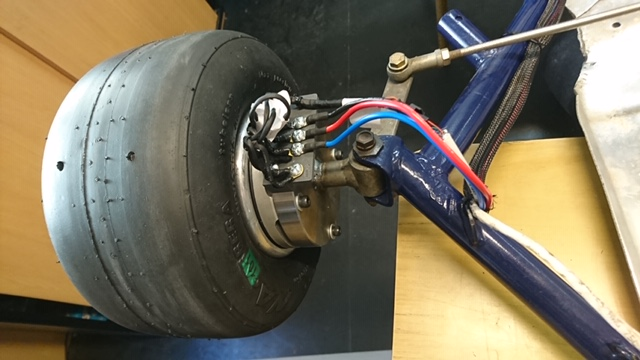
\includegraphics[width=0.5\textwidth]{figs/kart2.jpg}
    \caption{Detalle de partes}
    \label{fig:kart2}
\end{figure}

Los convertidores fueron diseñados y construidos en el Centro de investigación y Desarrollos en Electrónica Industrial (CIDEI) y se encuentran montados en la parte trasera del vehículo. Los mismos fueron dimensionados en función de las especificaciones de los motores traseros, los cuales son de una potencia 10 veces superior a los delanteros y todavía en la fase actual en la que se encuentra el proyecto no se encuentran instalados.

De momento el proyecto se encuentra en una fase preeliminar donde se validará el diseño y la mecánica del karting con tracción delantera únicamente. La siguiente fase del proyecto incluye la colocación e instalación de los motores traseros junto con su electrónica asociada y el reacomodamiento de las baterías y la electrónica en los laterales del vehículo. En esta etapa será necesario incorporar un freno mecánico extra ya que el eje trasero será independiente para cada rueda y es necesario un mecanismo de seguridad físico con el cual detener al vehículo.

Este proyecto se vincula con otros proyectos en progreso, ya sea porque se utilizan en la electrónica del vehículo, como la placa de FPGA libre, o porque son necesarios para la versión final del prototipo como la placa de Arduino con comunicación CAN.

\subsection{Etapas de desarrollo}
Se dividió al proyecto en varias etapas, donde la etapa 1 está finalizada y la etapa 2 se encuentra en ejecución. Estas etapas y una breve descripción de las tareas asociadas a las mismas se detallan a continuación.
\begin{enumerate}
    \item Desarrollo de especificaciones y compra de motores
    \begin{itemize}
        \item En esta etapa se definen las especificaciones de funcionamiento del karting y se realiza la compra de los motores ya que por falta de especificaciones completas de los mismos son necesarios para el diseño de las piezas que se requieren construir \par FINALIZADO
    \end{itemize}
    \item Diseño, construcción y verificación de la electrónica necesaria
    \begin{itemize}
        \item Se desarrollan los convertidores electrónicos de potencia para los motores y también la electrónica asociada a los sensores externos. \par Convertidores: FINALIZADO, Placa A2CAN: EN CONSTRUCCIÓN
    \end{itemize}    
    \item Tracción Delantera
    \begin{itemize}
        \item Se incorporarán los motores eléctricos delanteros y se desarrollarán las primeras pruebas de funcionamiento en condiciones reales \par EN PROCESO
    \end{itemize}
    \item Tracción Trasera
    \begin{itemize}
        \item Se incorporarán los motores eléctricos traseros y se validará el funcionamiento
    \end{itemize}    
    \item Tracción Integral
    \begin{itemize}
        \item Aplicando técnicas de control se validarán las mejoras esperadas al contar con tracción integral
    \end{itemize}    
    \item Incorporación de baterías de última generación
    \begin{itemize}
        \item Los vehículos eléctricos actualmente se desarrollan en base a baterías de Litio ion, las cuales poseen un gran rendimiento en bajo volumen pero son costosas y requieren hardware específico para su utilización \par BUSCANDO FINANCIAMIENTO
    \end{itemize}    
    \item Trabajos de Investigación
    \begin{itemize}
        \item Realizar trabajos de investigación basados en la experiencia recolectada, utilizando la plataforma desarrollada para la obtención de resultados experimentales
    \end{itemize}    
\end{enumerate}

\subsection{Personal}
El equipo de trabajo está compuesto por varias personas:
\begin{itemize}
    \item Dr. Miguel Aguirre - Director del Dpto. de Eléctrica y Electrónica
    \item Dr. Pablo Cossutta - Director del CIDEI
    \item Dr. Alejandro Ghersin - Especialista en el área de Control
    \item Ing. Juan Matus - Técnico asociado a tareas de investigación
    \item Jorge Cáceres - Técnico asociado a tareas de soporte del Dpto.
    \item Milagros Moutín - Becarias Ing. Electrónica
    \item Pablo Gonzalez - Becario Ing. Electrónica
    \item Marcos Brito Devoto - Alumno Ing. Electrónica
    \item Gonzalo Castelli - Alumno Ing. Electrónica, desarrolló su pasantía laboral en el CIDEI en tareas relacionadas con el proyecto
    \item Ing. Juan Talpone - Ex. miembro del CIDEI, trabajó en el desarrollo de los convertidores electrónicos de potencia
\end{itemize}

En las Fig. \ref{fig:equipo1}, Fig. \ref{fig:equipo2} y Fig. \ref{fig:equipo3} se observa a parte del equipo con el karting y realizando trabajos sobre la plataforma.
%
\begin{figure}[h]
    \centering
    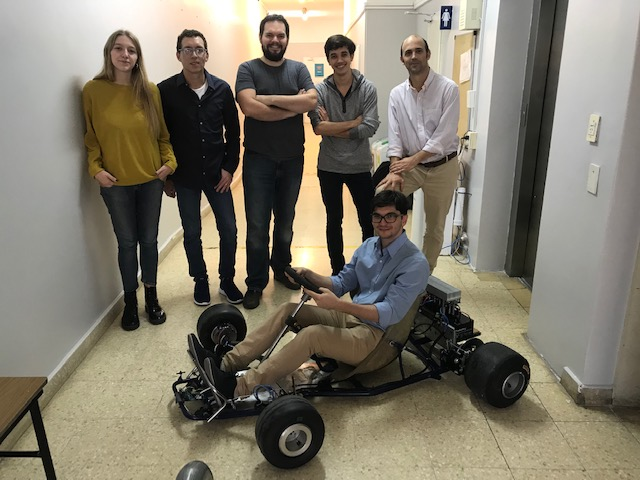
\includegraphics[width=0.7\textwidth]{figs/equipo1.jpg}
    \caption{Parte del equipo de trabajo}
    \label{fig:equipo1}
\end{figure}
%
\begin{figure}[h]
    \centering
    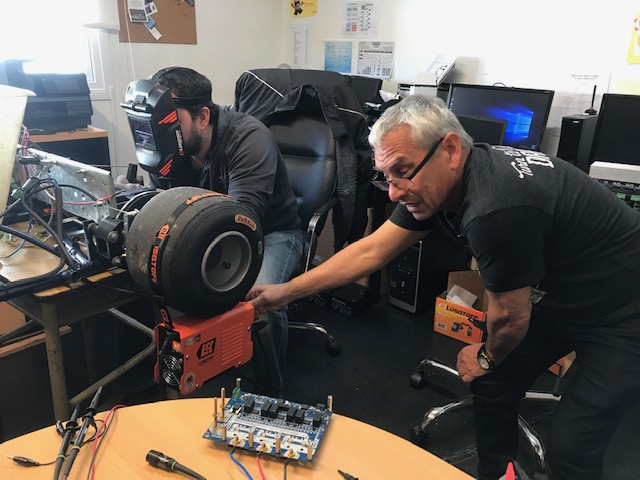
\includegraphics[width=0.4\textwidth]{figs/equipo2.jpg}
    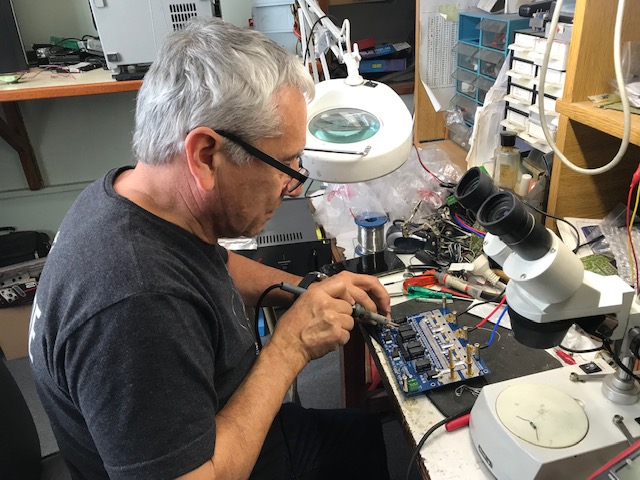
\includegraphics[width=0.4\textwidth]{figs/equipo3.jpg}
    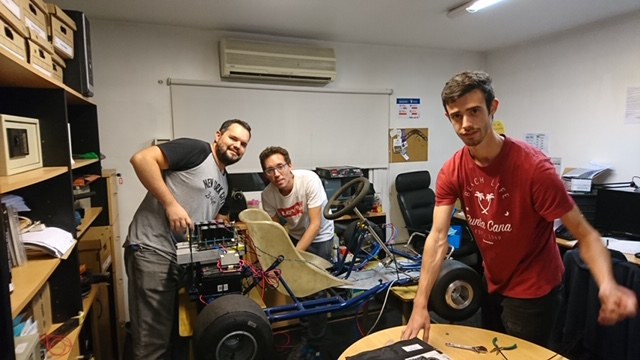
\includegraphics[width=0.6\textwidth]{figs/equipo4.jpg}
    \caption{Trabajos mecánicos y eléctricos}
    \label{fig:equipo2}
\end{figure}
%
\begin{figure}[h]
    \centering
    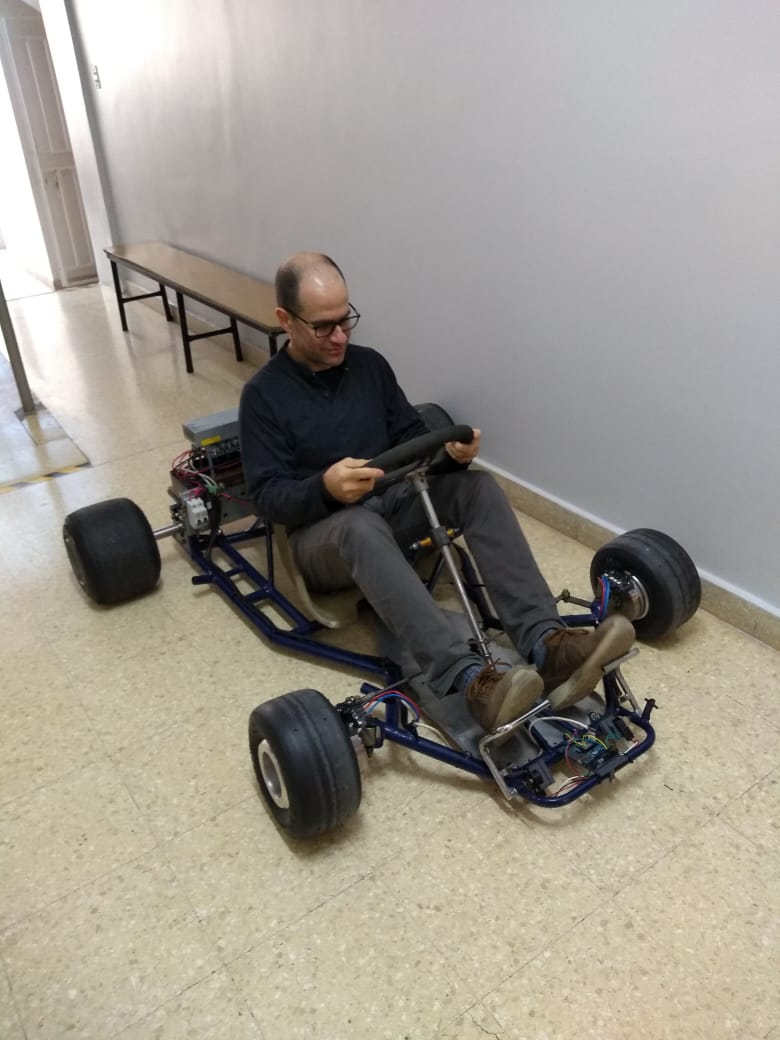
\includegraphics[width=0.45\textwidth]{figs/equipo5.jpg}
    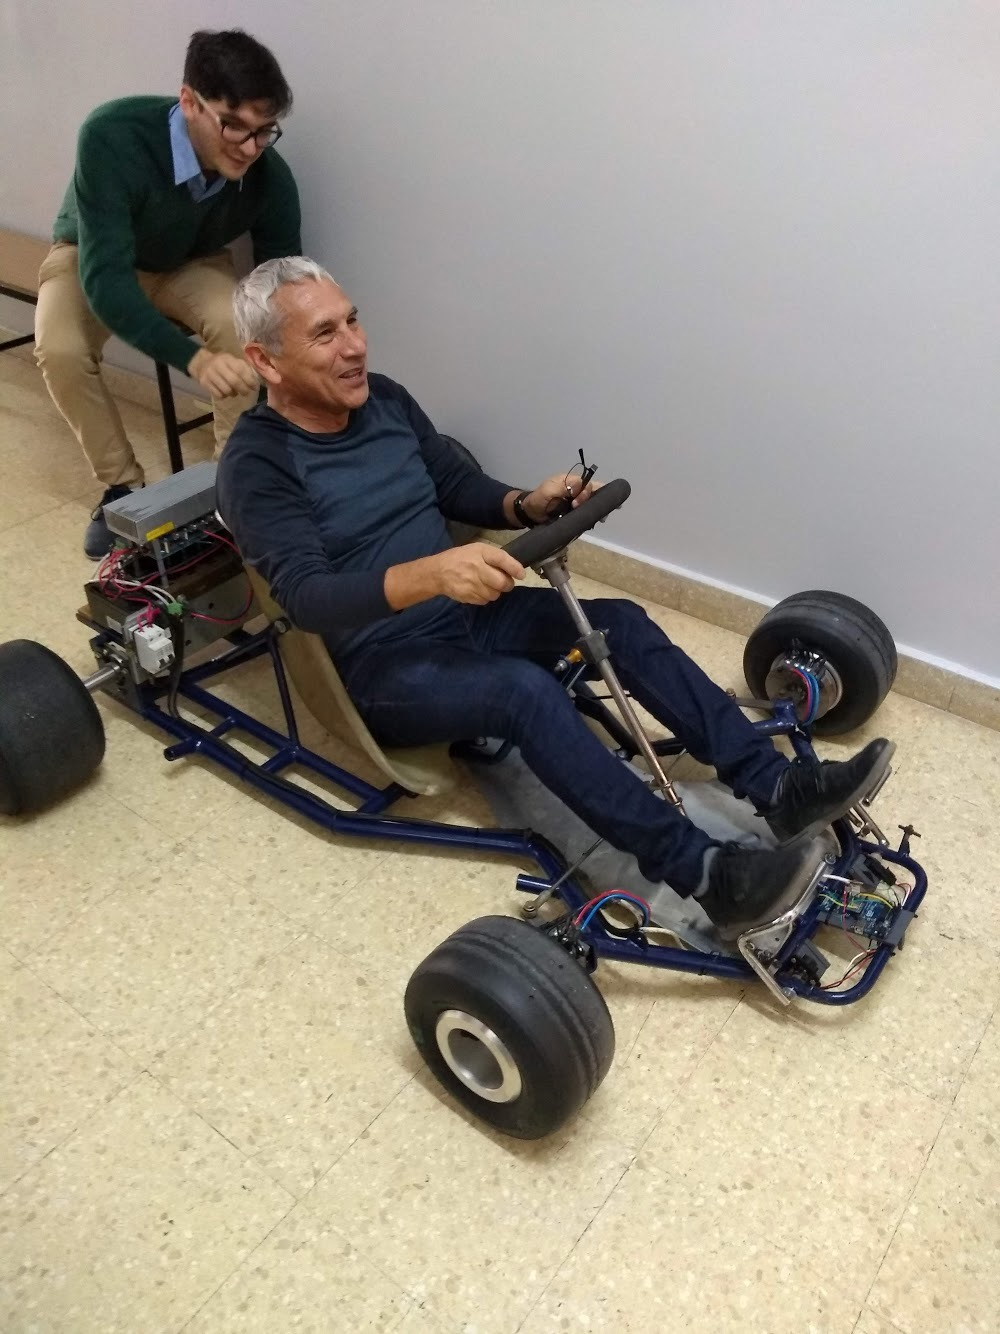
\includegraphics[width=0.45\textwidth]{figs/equipo6.jpg}
    \caption{Prueba de manejo}
    \label{fig:equipo3}
\end{figure}

\section{FPGA}
Este proyecto, el cual se utiliza en los convertidores utilizados para controlar los motores del karting fue desarrollado en el CIDEI en conjunto con becarios y alumnos desarrollando su pasantía laboral.
El mismo consta del desarrollo de una plataforma experimental para el uso y aprendizaje de FPGA de bajo costo y totalmente libre, la cual puede observarse en la Fig. \ref{fig:fpga}. El hardware (Desarrollado y validado en el ITBA) será libre y existen herramientas de software para utilizar en los procesos de síntesis, implementación, validación y programación, también libres como por ejemplo la plataforma libre creada por by Clifford Wolf, \href{http://www.clifford.at/icestorm/}{Project IceStorm}.
%
\begin{figure}[h]
    \centering
    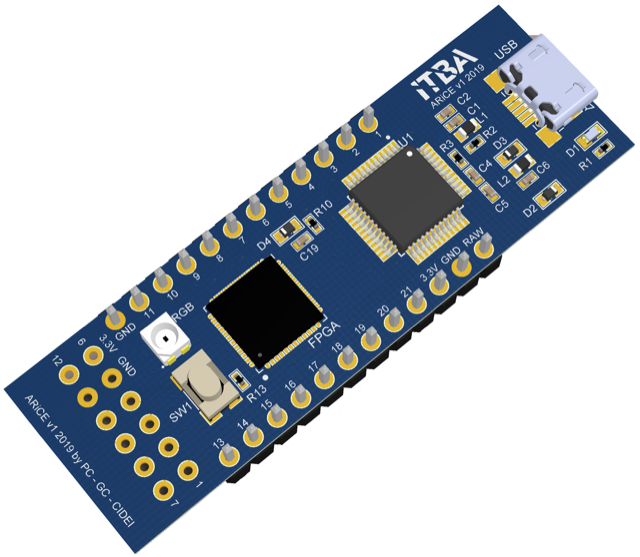
\includegraphics[width=0.4\textwidth]{figs/fpga1.png} \\
    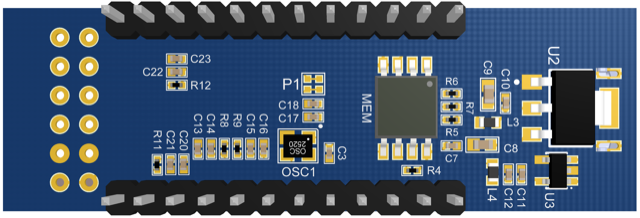
\includegraphics[width=0.4\textwidth]{figs/fpga2.png}
    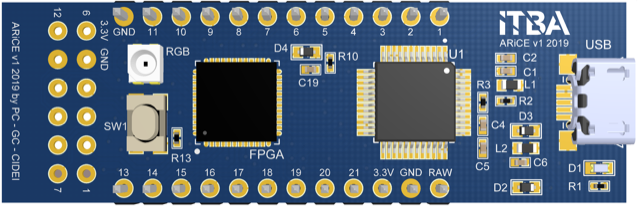
\includegraphics[width=0.4\textwidth]{figs/fpga3.png}
    \caption{FPGA}
    \label{fig:fpga}
\end{figure}

La plataforma desarrollada también se combina con el software de la firma Lattice, el cual se utiliza para programar el chip iCE40-UP5K,  \href{http://www.latticesemi.com/Products/DesignSoftwareAndIP/FPGAandLDS/Radiant}{Lattice Radiant}. Este software soporta las versiones iCE40 UltraPlus de la familia de FPGAs y provee una forma de desarrollar aplicaciones en forma efectiva y eficiente con soporte directo del fabricante.

El objetivo es crear un ecosistema libre donde existan múltiples ejemplos de uso, tutoriales y videos de iniciación con el fín de fomentar el uso y aprendizaje de estas tecnologías. Está previsto comenzar a desarrollar cursos basados en la plataforma y asimismo utilizarla en las materias pertinentes de la carrera de Ing. Electrónica.

El proyecto está próximo a concluir y en breve se estará liberando al público como un repositorio de Github con el fin de contribuir a la comunidad.

\section{Arduino-CAN}
Este otro proyecto, combina la facilidad de programación de la plataforma \href{http://arduino.cc}{Arduino} con los beneficios de la comunicación mediante CAN, tecnología ampliamente adoptada en la industria automotriz. El objetivo es desarrollar una plataforma, como la que se observa en la Fig. \ref{fig:a2can}, de fácil utilización que permita adquirir datos de sensores externos y comunicar mediante protocolo CAN sus valores. El desarrollo ha sido completado en el CIDEI mediante un alumno que ha realizado parte de su pasantía laboral en el CIDEI, y actualmente está siendo construido para ser incorporado al vehículo.
%
\begin{figure}[h]
    \centering
    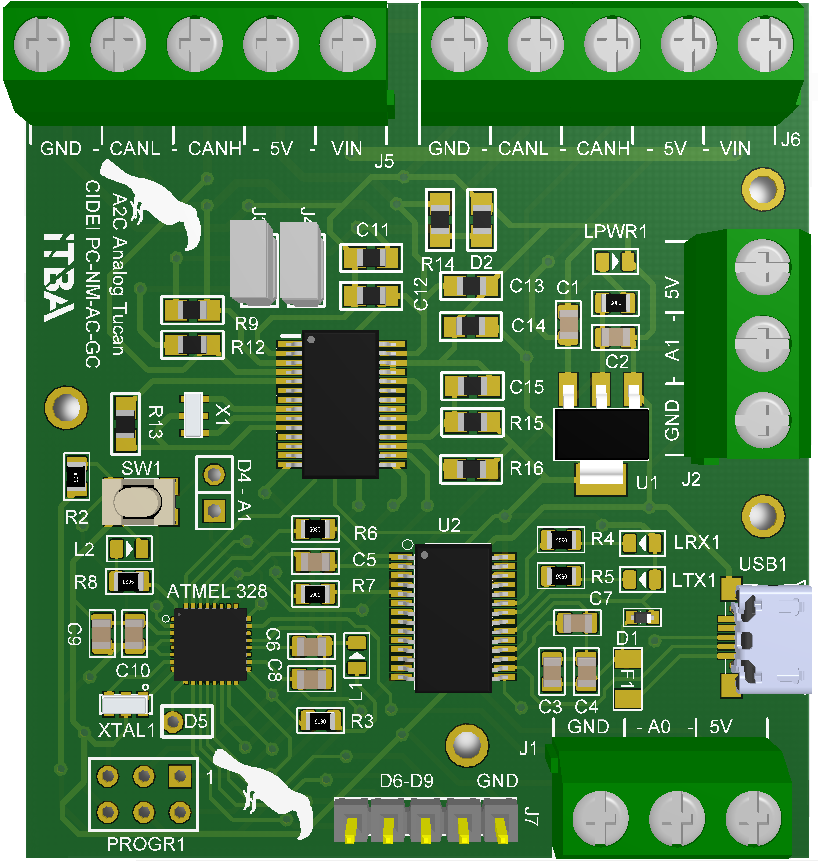
\includegraphics[width=0.35\textwidth]{figs/a2can.png}
    \caption{Plataforma A2CAN}
    \label{fig:a2can}
\end{figure}

Este circuito permitirá añadir diversos sensores de una forma simple y sistemática al proyecto.

\section{Información Adicional}
En el siguiente enlace de Google Drive\texttrademark \space se incluyen imágenes adicionales y vídeos de algunas de las pruebas de conducción realizadas. 

\href{https://drive.google.com/drive/folders/1y7x4eIJOVqtQwzSrL0hkvnH02-Jpi3-s?usp=sharing}{https://drive.google.com/drive/folders/1y7x4eIJOVqtQwzSrL0hkvnH02-Jpi3-s?usp=sharing}

\end{document}
